\documentclass[tikz,border=8pt]{standalone}
% Shared look for every TikZ diagram. Load with \input{../../tools/tikz-style.tex}
\usepackage[T1]{fontenc}
\usepackage{lmodern}
\renewcommand{\sfdefault}{lmr}  % diagrams use the same serif as the text
\usetikzlibrary{arrows.meta, positioning, shapes.geometric, calc, fit, backgrounds}
\definecolor{cblue}{HTML}{4C78A8}
\definecolor{corange}{HTML}{F58518}
\definecolor{cgreen}{HTML}{54A24B}
\definecolor{cred}{HTML}{E45756}
\definecolor{cpurple}{HTML}{B279A2}
\definecolor{cgrey}{HTML}{6B6B6B}
\tikzset{
  every picture/.style={font=\sffamily, line width=1.2pt},
  box/.style={draw=#1, fill=#1!12, rounded corners=4pt, align=center, inner sep=7pt, minimum height=1.1cm},
  box/.default=cgrey,
  arrow/.style={-{Stealth[length=3mm]}, draw=cgrey, line width=1.4pt},
  title/.style={font=\sffamily\bfseries\Large},
  note/.style={font=\sffamily\small, text=cgrey, align=center},
}
\AtBeginDocument{\hyphenpenalty=10000 \exhyphenpenalty=10000}

% Section 4: step 0 once, then steps 1-4 for each student, with student 1's numbers.
\begin{document}
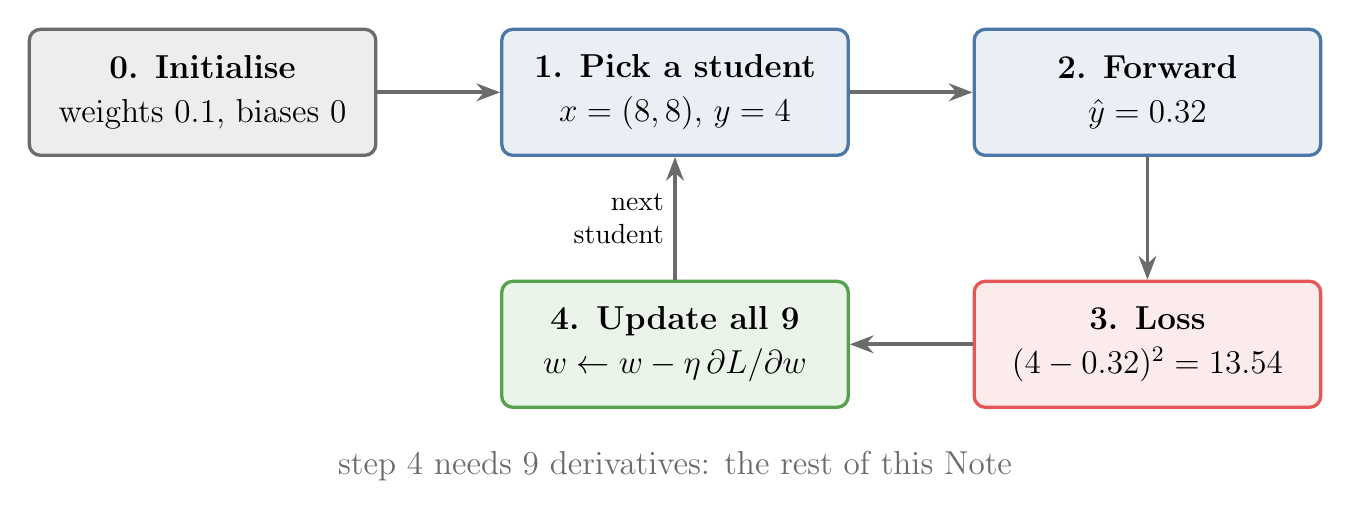
\begin{tikzpicture}[s/.style={box=#1, minimum width=4.4cm, minimum height=1.6cm, font=\large},
                    num/.style={font=\normalsize, text=cgrey}]
  \node[s=cgrey] (s0) at (0, 0) {\textbf{0. Initialise}\\[2pt] weights 0.1, biases 0};
  \node[s=cblue] (s1) at (6, 0) {\textbf{1. Pick a student}\\[2pt] $x = (8, 8)$, $y = 4$};
  \node[s=cblue] (s2) at (12, 0) {\textbf{2. Forward}\\[2pt] $\hat y = 0.32$};
  \node[s=cred] (s3) at (12, -3.2) {\textbf{3. Loss}\\[2pt] $(4 - 0.32)^2 = 13.54$};
  \node[s=cgreen] (s4) at (6, -3.2) {\textbf{4. Update all 9}\\[2pt] $w \leftarrow w - \eta\,\partial L/\partial w$};
  \draw[arrow] (s0) -- (s1);
  \draw[arrow] (s1) -- (s2);
  \draw[arrow] (s2) -- (s3);
  \draw[arrow] (s3) -- (s4);
  \draw[arrow] (s4) -- node[left, font=\normalsize, align=right] {next\\student} (s1);
  \node[note, font=\large] at (6, -4.75) {step 4 needs 9 derivatives: the rest of this Note};
\end{tikzpicture}
\end{document}
